\section{Material y Métodos} \label{sec:material}

\subsection{Vision General del Sistema}

Se ha definido un pipeline de ejecución que permite realizar múltiples experimentos de forma iterativa y automatizada. Este pipeline está compuesto por distintos módulos encargados de gestionar el preprocesamiento de los datos, la configuración de los modelos, el entrenamiento y la evaluación de los mismos.

Con el objetivo de facilitar la reproducibilidad y la exploración sistemática de parámetros, el código se ha estructurado como un microframework que permite modificar de forma sencilla las variables de estudio, así como controlar la ejecución de los experimentos. Este enfoque ha resultado especialmente útil dado el elevado número de ejecuciones.

Para organizar la ejecución, se ha definido una estructura jerárquica en tres niveles:

\begin{itemize}
    \item \textbf{Experimento}: nivel superior que agrupa el conjunto completo de configuraciones evaluadas. Un experimento consiste en la ejecución sistemática de múltiples combinaciones de parámetros.
    \item \textbf{Iteración}: cada una de las ejecuciones individuales del pipeline dentro de un experimento, asociada a una combinación específica de parámetros (arquitectura, método de entrenamiento y tipo de tarea).
    \item \textbf{Entrenamiento}: nivel más bajo de la jerarquía, correspondiente al entrenamiento y evaluación de un modelo para un usuario y sesión concretos dentro de una iteración.
\end{itemize}

De este modo, cada experimento está compuesto por múltiples iteraciones, y cada iteración incluye varios entrenamientos, uno por cada usuario y sesión del dataset.
Los experimentos se definen mediante la combinación de distintos parámetros, entre los que destacan el tipo de tarea, la arquitectura del modelo y el método de entrenamiento. Para cada combinación se ejecuta una iteración independiente

En cada iteración, el sistema inicializa los parámetros de entrenamiento y carga el conjunto de datos correspondiente al tipo de tarea. A continuación, se ejecuta el método de entrenamiento seleccionado, en el que se itera sobre los distintos usuarios y sesiones disponibles en el dataset. Para cada caso, se inicializa el modelo, se realiza el entrenamiento y se evalúa su rendimiento.

Finalmente, los resultados obtenidos, junto con los parámetros utilizados, se almacenan de forma estructurada, permitiendo su posterior análisis. 

Este proceso permite realizar un estudio posterior de los resultados obtenidos por cada combinación de parámetros definida.

La Figura \ref{fig:pipeline_general} resume la organización jerárquica del pipeline experimental.

\begin{figure}[H]
    \centering
    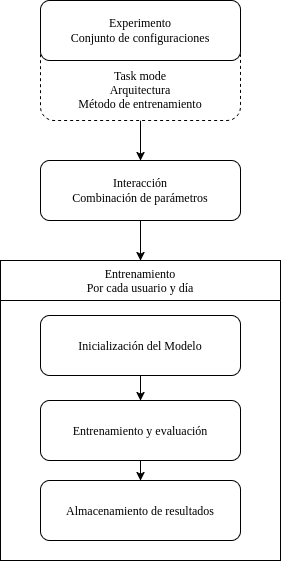
\includegraphics[width=0.45\textwidth]{img/diagrama_pipeline.drawio.png}
    %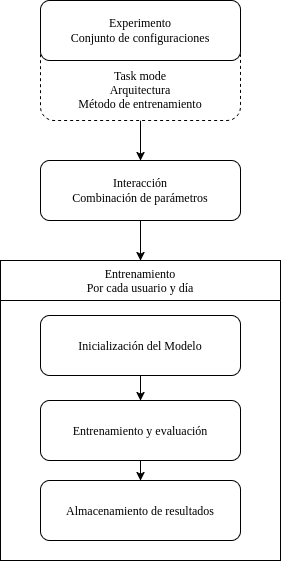
\includegraphics[height=\dimexpr\pagegoal-\pagetotal-\baselineskip\relax,width=\textwidth,keepaspectratio]{img/diagrama_pipeline.drawio.png}
    \caption{Pipeline experimental}
    \label{fig:pipeline_general}
\end{figure}

\subsection{Materiales}
\subsubsection{Hardware}

Para ejecutar los distintos entrenamientos se ha utilizado un ordenador con las siguientes características:

\begin{itemize}
    \item \textbf{CPU}: Intel Core i9-14900HX
    \item \textbf{RAM}: 31 GiB
    \item \textbf{GPU}: NVIDIA GeForce RTX 4060
    \item \textbf{GPU RAM}: 8 GiB
\end{itemize}

Estas características han resultado suficientes para completar los experimentos planteados sin limitaciones críticas. 
El tiempo medio de entrenamiento por iteración ha sido aproximadamente 40 minutos, dependiendo de la configuración del modelo y de los parámetros de entrenamiento. 

El tiempo total de cómputo se estima mediante:


\begin{equation*}
    \text{Tiempo total (h)} = \frac{N_{\text{iteraciones}} \times t_{\text{iteración}}}{60}
\end{equation*} 

Donde $N_{\text{iteraciones}} = 1917$ y $t_{\text{iteración}} = 40 \text{minutos}$, resultando en un tiempo total aproximado de 766.8 horas ($\approx 31 \text{días}$).

El uso de hardware con mayores prestaciones permitiría reducir significativamente el tiempo total de entrenamiento y facilitar la realización de un mayor número de experimentos.

\subsubsection{Sofware}

Para el desarrollo del proyecto se ha utilizado una infraestructura basada en herramientas ampliamente empleadas en el ámbito del aprendizaje automático y la ingeniería de software.

Como lenguaje de programación principal se ha utilizado Python\footnote{https://www.python.org/}, debido a su amplio ecosistema de librerías científicas y de aprendizaje automático, así como su facilidad de integración con frameworks de alto nivel.

Para la construcción y entrenamiento de los modelos se han utilizado TensorFlow\footnote{https://www.tensorflow.org/} y Keras\footnote{https://keras.io/}, frameworks de aprendizaje profundo que permiten definir, entrenar y evaluar redes neuronales de forma eficiente. Keras se ha empleado como interfaz de alto nivel sobre TensorFlow, facilitando la experimentación rápida con distintas arquitecturas.

Durante las etapas iniciales del proyecto se empleó Jupyter Notebook\footnote{https://jupyter.org/} para la realización de pruebas exploratorias y la visualización preliminar de resultados. Sin embargo, su uso fue descartado en fases posteriores debido a la dificultad para mantener una estructura de código modular y escalable en experimentos de mayor complejidad.

Posteriormente, se adoptó Visual Studio Code\footnote{https://code.visualstudio.com/} como entorno de desarrollo principal, debido a su capacidad para gestionar múltiples tipos de archivos y su integración con herramientas de desarrollo. Se utilizaron extensiones específicas para Python, Jupyter y GitHub, permitiendo un flujo de trabajo unificado.

Como sistema de control de versiones se ha utilizado GitHub\footnote{https://github.com/}, que facilita la gestión del código, el seguimiento de cambios y la colaboración con el tutor del proyecto. Además, permite la sincronización del repositorio entre distintos dispositivos de forma eficiente.

Para la visualización de resultados se ha utilizado Vega-Altair\footnote{https://altair-viz.github.io/}, una librería de visualización estadística declarativa enfocada en la simplicidad, eficiencia y legibilidad. A diferencia de enfoques imperativos como Matplotlib, Altair permite definir visualizaciones de forma estructurada y reproducible, enfocándose en lo que se quiere observar en lugar de en los detalles de la implementación. Esto conduce a un código más limpio y legible\cite{geeks_altair_2025}.

Como gestor de base de datos se ha utilizado DuckDB\footnote{https://duckdb.org/}, un sistema de bases de datos analítico embebido que permite realizar consultas SQL de forma eficiente directamente sobre archivos locales. Su integración con Python y su alto rendimiento lo hacen especialmente adecuado para el procesamiento de grandes volúmenes de resultados experimentales\cite{duckdb_2026}.

Todas estas herramientas han sido integradas en un flujo de trabajo unificado orientado a la ejecución reproducible de experimentos.

\subsection{Estructura Dataset}

El dataset utilizado se compone por dos ficheros de labels y dos de datos de entrenamiento. Los labels contienen la intención de movimiento de cada canal de EEG, mientras que los datos contienen las lecturas de cada canal de EEG.

Estos ficheros están separados por la tarea a analizar, de esta forma tenemos los cuatro ficheros:

\begin{center}
    \begin{tabular}{|c|c|c|}
        \hline
         & \textbf{Labels} & \textbf{Training} \\ \hline
        \textbf{Static} &\texttt{labels\_static\_data.mat} & \texttt{training\_static\_data.mat} \\ \hline
        \textbf{Motion} &\texttt{labels\_motion\_data.mat} & \texttt{training\_motion\_data.mat} \\ \hline
    \end{tabular}
\end{center}

%% también puedo ponerlo así
\begin{itemize}
    \item \texttt{labels\_static\_data.mat}
    \item \texttt{training\_static\_data.mat}
    \item \texttt{labels\_motion\_data.mat}
    \item \texttt{training\_motion\_data.mat}
\end{itemize}

Los ficheros contienen la siguiente estructura de datos:
Los labels tienen la forma (15400, 1), mientras que los datos tienen la forma (15400, 27, 400).
Los ficheros de labels contienen una matriz con el numero de ventanas y una columna con la intención de movimiento
Los ficheros de training contienen una matriz de tamaño $N \times C \times S$, donde $N$ es el número de ventanas, $C$ es el número de canales y $S$ es el número de muestras. En el caso de este experimento $N = 15400$ $C = 27$ y $S = 400$. Las muestras son obtenidas durante 2 segundos a 200hz

%% ESTA PARTE ESTÁ Sacada del paper original de donde se sacan los datos
The 27 channels selected for acquisition were: F3, FZ, FC1, FCZ, C1, CZ, CP1, CPZ, FC5, FC3, C5, C3, CP5, CP3, P3, PZ, F4, FC2, FC4, FC6, C2, C4, CP2, CP4, C6, CP6, P4. They were placed following the 10-10 international system.
Four electrodes were located next to the eyes to record electrooculography (EOG) and ground and reference electrodes were located on the right and left ear lobes, respectively. Each channel signal was amplified with BrainVision BrainAmp amplifier. 

%NOSE COMO PONER ESTO:
Se tienen los datos de 5 usuarios, con 5 días cada uno, 11 trials por día, cada día, 56 ventanas por trial. Por lo tanto, se tienen 5 x 5 x 11 x 56 = 15400 ventanas.

Cada trial corresponde a una secuencia de dos tareas mentales, relajación e imaginación de la marcha, que se repite en intervalos de 14 ventanas temporales (0.5s x ventana = 0.7s) de relajación, 28 de imaginación de la marcha (0.5s x ventana = 1.4s) y finalmente otras 14 de relajación. 
Se cuenta con un periodo inicial de duración aleatoria en la cual se le pedía al sujeto realizar una tarea mental compleja, diferente a la imaginación motora. Este periodo se utiliza para eliminar ruidos en la señal EEG y se ha eliminado del dataset final.

Un esquema de las ventanas se puede ver en la figura \ref{fig:ventanas}.

\begin{figure}[H]
    \centering
    
\includegraphics[width=0.8\textwidth]{ventanas.png}
    \caption{Esquema de las ventanas}
    \label{fig:ventanas}
\end{figure}

Los labels y los datos están relacionados a nivel de ventana, utilizando un fichero auxiliar vector_tasks_training.mat.

\subsubsection{Preprocesamiento de datos}

Los datos han sido procesados previamente en otro estudio.
Para este trabajo, se modificaron los arrays para que tuvieran 6 dimensiones (input) y 5 dimensiones (labels):
input_6d = input_data.reshape(N_USERS,N_DAYS,N_TRIALS,N_WINDOWS,N_CHANNELS,N_SAMPLES)
labels_6d = labels_data.reshape(N_USERS,N_DAYS,N_TRIALS,N_WINDOWS,1)

La separación entre los datos de entrenamiento y testeo se ha hecho en un 70\% de entrenamiento y 30\% de testeo y se aplica al nivel de trial. Esta separación se ha hecho para cada entrenamiento del modelo y se toma en cuenta el usuario y día de cada uno. No se ha hecho de manera aleatoria, sino que se han utilizado para testeo empezando por el final de la lista de trials. 

La razón de esta decisión es que en los primeros trials el sujeto suele presentar un menor control sobre su imaginación motora. %esta frase no me gusta ni un pelooooooo

Más allá de estos preprocesamientos, no se ha hecho nada más

la Pipeline
qué hace tu sistema de principio a fin

Ejemplo:

    entrada: EEG

    procesamiento

    modelo

    salida: predicción


\subsection{Modelos utilizados}
Aquí metes:

\subsubsection{EEGNet}
\subsubsection{DeepConvNet}
\subsubsection{ShallowConvNet} (si lo usas)

Para cada uno:

    breve descripción (2–3 líneas)

    por qué lo eliges

NO pongas la arquitectura entera en detalle aquí (eso es más de anexos si acaso)

\subsection{Metodología experimental}

Aquí es donde entra todo tu proyecto de verdad.
\subsubsection{Variables del estudio}

Muy importante estructurarlo así:

    Arquitectura del modelo

    Método de entrenamiento:

        same-day

        acumulativo

        fine-tuning

    Tarea:

        static / motion

    Usuario

\subsubsection{Estrategia de entrenamiento}\label{sec:metodos_entrenamiento}

    epochs

    batch size

    callbacks:

        early stopping

        reduce LR

    función de pérdida

    métrica (accuracy)

No te líes demasiado, pero deja claro cómo entrenas



\subsubsection{Evaluación}

MUY importante:

    validación cruzada

    pseudo-online

explica qué significa pseudo-online (aunque sea breve)



\subsection{Infraestructura Experimental}

Aquí metes tu microframework (esto es TU aporte técnico fuerte)

sistema para ejecutar múltiples experimentos
gestión de parámetros
almacenamiento de resultados (DuckDB)
automatización

Esto es diferencial → véndelo bien


Se ha programado un microframework para el desarrollo de experimentos de Machine Learning.

Como se ha comentado en el apartado \ref{sec:}, se ha realizado la comparación de tres modelos de redes neuronales convolucionales para la clasificación de la intención de caminar o detenerse con un exoesqueleto. Se ha utilizado un dataset de EEG con 27 canales, obtenido de una muestra de un estudio previo XXXXXX. Los parametros a comparar son la arquitectura de la red, el metodo de entrenamiento, la tarea a predecir y la variabilidad entre usuarios.

Al necesitarse de cientos de ejecuciones para obtener todos los datos necesarios, durante las etapas iniciales se tomó la decisión de enfocar el proyecto de manera horizontal, preparando una base de ejecución sobre la cual modificar facilmente todo lo necesario para cada ejecución y permitiendo ejecutar multiples experimentos de manera secuencial.

(((((((Aquí no sé si ir diicendo TOOOOODo lo que he ido poniendo en el código. Puedo ir siguiendo el timeline de Github y hacer un resumen de los commits))))))))


\subsubsection{Diseño de experimentos}

Aquí explicas cómo organizaste TODO

combinaciones de parámetros
nº de ejecuciones
cómo comparas resultados

Esto conecta directamente con Results luego